\chapter{Theory and motivation}
\label{sec:Theory}

\section{The Standard Model of Particle Physics}
The Standard Model of particle physics (SM) is a relativistic and renormalisable quantum field theory, that combines the electroweak theory developed by Glashow, Salam and Weinberg \cite{SM_Glashow, SM_Salam, SM_Weinberg} with quantum chromodynamics (QCD), the theory of the strong interactions.
It combines the current knowledge of fundamental particles and their interactions at microscopic level with the exception of gravitation.

The electroweak theory is already a combination of the electromagnetic and the weak interaction.
Every fundamental particle can interact via the weak force.
For instance, the weak force is responsible for the $\beta$-decay of neutrons.
Atoms or molecules are bound by the electromagnetic interaction taking place between electrically charged particles.
If particles also carry a so-called colour charge, they can interact via the strong interaction, which binds e.g. protons and neutrons in a nucleus.

In the Standard Model, matter arises as half-integer spin particles from quantum fields.
These particles are called \textsc{Fermions} and can be furthermore split up in \textsc{Quarks} and \textsc{Leptons}.
There exist 6 so-called ``flavours" of quarks: up (\uquark), down (\cquark), charm (\cquark), strange (\squark), top (\tquark) and bottom\footnote{The bottom quark is sometimes also called beauty.} (\bquark).
According to their mass and other physical properties, they can be grouped into three generations:
\begin{align*}
    \begin{pmatrix} \uquark \\ \dquark \end{pmatrix},
    \begin{pmatrix} \cquark \\ \squark \end{pmatrix},
    \begin{pmatrix} \tquark \\ \bquark \end{pmatrix}.
\end{align*}
Quarks in the top row are referred to as \textsc{Uptype} quark.
They carry an electrical charge of $+\frac{2}{3}e$, whereas \textsc{Downtype} quarks carry a charge of $-\frac{1}{3}e$.
Thus, they can participate in the electromagnetic interaction.
In addtion, quarks carry colour charge allowing them to interact via the strong interactions.

Leptons do not carry flavour as opposed to quarks.
There exist three flavours of leptons, namely the electron (\en), the muon (\mun) and the tauon (\taum) with an electric charge of $-e$ and their neutral counterparts, the neutrinos \neue, \neum, \neut.
Similarly to quarks, the leptons can be grouped into three generations
\begin{align*}
    \begin{pmatrix} \en \\ \neue \end{pmatrix},
    \begin{pmatrix} \mun \\ \neum \end{pmatrix},
    \begin{pmatrix} \taum \\ \neut \end{pmatrix}.
\end{align*}
As the neutrinos do neither carry electrical nor colour charge, they only interact weakly.
Due to that fact it is not possible to detect neutrinos at hadron colliders like the \lhc.
For each fermion, there exists a corresponding antifermion with same mass, but opposite quantum numbers.

In the Standard Model, the interactions among the particles are described by the mediation of spin-1 gauge bosons.
For the electromagnetic interaction, this is the electric neutral photon \g.
It couples to electrically charged particles.
Since the photon is massless the range of the electromagnetic interaction is infinite.
The weak interaction is mediated by three massive gauge boson.
The electrically charged \Wp and \Wm as well as the neutral \Z boson.
The \Wpm bosons only couple to left-handed fermions (or right-handed antifermions), whereas the \Z couples to both, left- and right-handed fermions, but with different strength.
Due to their large mass of $m_{\Wpm} \approx 80 \gev$ and $m_\Z \approx 91 \gev$ the weak interaction is only short-ranged.
The strong interaction is carried by 8 massless gluons.
They couple to particles carrying a colour charge and carry colour itself.
Thus, there is also a gluon-gluon coupling possible leading to a QCD coupling strength \as, which strongly depends on the momentum transfer in an interaction.
For low energies \as increases dramatically, which means that coloured particles cannot be isolated.
This phenomenon is called \textsc{Confinement}.
At high energies \as is very small resulting in the \textsc{Asymptotic Freedom}, i.e. the quarks are thus quasi-free while keeping short distances.
Due to the confinement, \textsc{Hadrons}, strongly interacting composite particle, must always be colour-neutral.
They exist either as quark-antiquark system and are called \textsc{Mesons} or as composite of three quarks and are named \textsc{Baryons}.
Recent \lhcb measurements report the observation of candidates for bound states consisting of 4 quarks (2 quark, 2 antiquarks) \cite{Tetraquark} and also 5 quarks (4 quarks, 1 antiquark) \cite{Pentaquark}.

Contradicting to the properties of the particles mentioned above, the invariance of local gauge transformation requires that the particles of the Standard Model are massless.
This problem is solved by the \textsc{Higgs mechanism}, which introduces a doublet of complex scalar (spin 0) fields.
The potential of thies field spontaneously breaks the electroweak symmetry and leads to massive bosons and fermions due to interaction with the Higgs field.
The Higgs mechanism furthermore predicts a massive spin-0 particle, the \textsc{Higgs Boson}.
As lastly unobserved particle, its discovery in July 2012 by \atlas \cite{Higgs_ATLAS} and \cms \cite{Higgs_CMS} was a big success for the experimental community as well as for the theory of the Standard Model itself. 
Figure \ref{fig:SM} summarises the fermions and bosons of the Standard Model and list their main properties \cite{Perkins_HEP, Burgess_SM, Meissner}.
\begin{figure}[ptb]
    \centering
	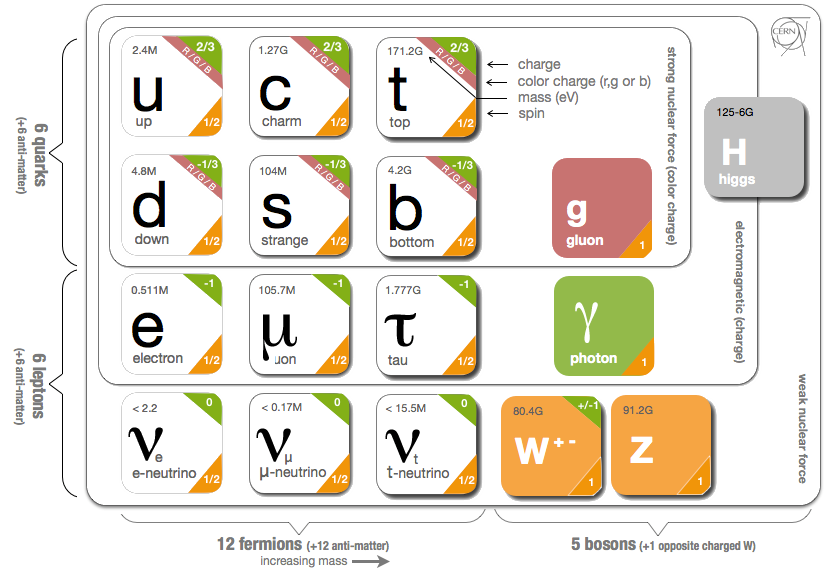
\includegraphics[width=\textwidth]{Standard_Model}	
	\caption{Summary of all fundamental fermions and bosons of the Standard Model of particle physics with their most important properties. Figure slightly modified and taken from \cite{SM_figure}.}
	\label{fig:SM}
\end{figure}

\section{The interest in \LbToDpmunuX}
There are several reasons why the study of the decay \LbToDpmunuX is interesting.
On the one hand the \Dz\proton subsytem allows spectroscopical studies to learn more about QCD, on the other hand the decay is a background in studies sensitive to physics beyond the Standard Model and thus limiting their precision.
This section ought to briefly introduce the areas and studies where a better understanding of \LbToDpmunuX is helpful.

\subsection{Baryonic spectroscopy}
There are plenty of combinatoric possibilities to combine three quarks to a baryon.
The constituent quark model predicts seven ground-state baryons with a total angular momentum $J$ and parity $P$ of $J^P = \frac{1}{2}^+$ containing a heavy \bquark quark and two light (\uquark, \dquark, \cquark) quarks: 
The \Lb singlet, the $\Sigma_b$ triplet, the $\Xi_b$ doublet and the \Omegab \cite{LHCb_Dph}.
Except for the $\Sigma_b^0$ all these states have been observed.
However the current knowledge of their fundamental properties like masses, widths and quantum numbers is poor as well as only few decay channels have been measured.
Thus, there is a big interest in the study of \bquark baryons.
The \Lb, which is studied in this analysis, has a quark content of \uquark\dquark\bquark and is the lightest \bquark baryon with a mass of $(5619 \pm 0.4) \mev$ \cite{PDG}.
Hence, it can only decay weakly as the strong and the electromagnetic interaction forbid quark transitions into other flavours.
This results in a characteristic, relatively long lifetime of $(1.451 \pm 0.013)\ps$ \cite{PDG}, which is helpful for the detection and reconstruction as will be explained later.

With the transition from a \bquark to a \cquark by the emission of a \Wm boson the \Lb can decay into a \Lc baryon.
The quark content of the \Lc is \uquark\dquark\cquark and thus a representative of a rich spectrum of \textsc{charmed baryons}.
Figure \ref{fig:Lc_spectrum} shows all known charmed baryons with their quantum number $J^P$ and their observed decays.
\begin{figure}[ptb]
    \centering
	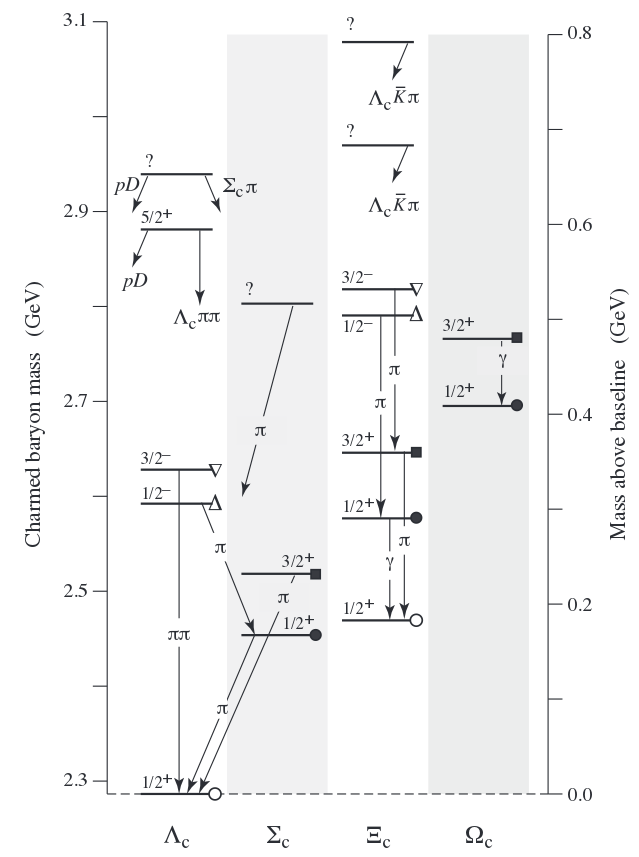
\includegraphics[width=\textwidth]{Lc_spectrum}	
	\caption{Summary of all known and established charmed baryons with quantum numbers $J^P$ and their observed decays. Figure taken from \cite{PDG}.}
	\label{fig:Lc_spectrum}
\end{figure}
Again, this spectrum is not complete.
A lot of expected charmed baryons are not established and also quantum numbers etc. of established charmed baryons have not been measured so far.
In 2006, \babar reported the observation of the charmed baryon decays \decay{\LcResI}{\Dz\proton} and \decay{\LcResII}{\Dz\proton} \cite{BaBar_D0p}.
Thus the decay \LbToDpmunuX, studied in this thesis offers the possibility to study \Lc resonances above the \Dz\proton mass threshold of $2803\mev$ by investigating the \Dz\proton subsystem.

The charmed baryon spectrum in Figure \ref{fig:Lc_spectrum} reminds of the emission spectrum of a hydrogen atom.
While the electromagnetic force is responsible for the splitting of the hydrogen's energy levels the spectroscopy of baryons offers the possibility to better understand QCD, the theory of the strong interaction.
Thus, QCD should be able to describe the dynamics of the baryons and predict their masses.
However, due to the rising coupling strength \as at short distances, QCD cannot treated perturbatively in the context of baryons.
Thus, there exist different approaches trying to solve QCD problems not generally, but at least under certain conditions.
Examples for such approaches are Lattice QCD \cite{LatticeQCD} or effective theories like the Heavy Quark Effective Theory (HQET) \cite{HQET_Introduction}.
The latter one has proven to be useful by the description of $b$ hadrons.
The main principle is that one considers the heavy $b$ quark as static source of the gluon field surrounded by the light quarks.
The theoretical simplification in describing the dynamics is analogous to consider a hydrogen atom instead of a positronium \cite{HQET_Introduction}.

\subsection{The hunt for New Physics at \lhcb}
It has already been stated in the introduction, that the Standard Model does not cover and explain all observed phenomena.
For instance, gravitation is not included in the Standard model, it does not provide a candidate for dark matter as well as dark energy and the asymmetry between matter and antimatter in the Standard Model is not large enough to fully explain why matter and animatter have not fully annihilated after
the big bang.
All physics that go beyond the Standard Model and try to answer those questions are generally referred to as \textsc{New Physics (NP)}.

In principle, there are two ways to discover New Physics:
The first one is to directly search for new particles.
This is what \atlas and \cms are doing and what lead to the discovery of the Higgs boson in 2012 \cite{Higgs_ATLAS, Higgs_CMS}.
However, one can only discover particles with a mass less than the available centre-of-mass energy \sqs.

The \lhcb way of searching for New Physics is an indirect one by the investigation of loop processes such as the \B/\Bbar mixing\footnote{A brief introduction of meson mixing will follow in the next sections.} shown in Figure \ref{fig:Bmixing}.
The virtual particles in the loops do not need to satisfy Einstein's energy momentum relation and thus can have heavier masses than the initial and final state particles.
Regarding the \B mixing, it is dominated by the top quark with a mass of $m_t = 173.3 \gev$ in the loop though the \B mass is only $m_\B = 5.3\gev$.
Thus, by a precise measurement of the \B meson mixing one is sensitive to a particle with a mass more than 30 times higher than the \B mass and hence the necessary center of mass energy needed for its production.
If there exists new heavy particles they might also contribute to such loop processes.
By a precise measurement of them, \lhcb tries to find deviations from Standard Model predictions for some variables.
Two of them, \asld and \Vub will be introduced in the following.
\begin{figure}[ptb]
    \centering
	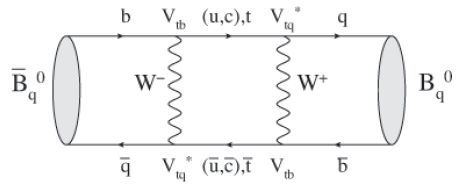
\includegraphics[width=0.6\textwidth]{bmixing}	
	\caption{One possible Feynman diagram for \B/\Bbar mixing. The \quark denotes either a \dquark or an \squark quark. Figure taken from \cite{LHCb_roadmap}.}
	\label{fig:Bmixing}
\end{figure}

\section{Flavour physics and the measurement of $|\Vub|$}
The flavour eigenstates of the weak interaction \ket{\dquark'},\ket{\squark'},  \ket{\bquark'} are not equal to the mass eigenstates \ket{\dquark},\ket{\squark},  \ket{\bquark}.
The transformation between those eigenstates is described by the unitary \textsc{Cabibbo-Kobayashi-Maskawa (CKM) matrix} $V_\text{CKM}$ \cite{Kobayashi_CKM}:
\begin{align}
\begin{pmatrix}
\ket{d'} \\ \ket{s'} \\ \ket{b'}
\end{pmatrix}
=
\begin{pmatrix}
V_{ud} & V_{us} & V_{ub} \\
V_{cd} & V_{cs} & V_{cb} \\
V_{td} & V_{ts} & V_{tb} \\
\end{pmatrix}
\cdot
\begin{pmatrix}
\ket{d} \\ \ket{s} \\ \ket{b}
\end{pmatrix}.
\end{align}
The probability that a quark with a mass eigenstate \ket{j} decays into a quark with mass eigenstate \ket{i} is given by $|V_{ij}|^2$.
As the CKM matrix is complex there are in principle 18 free parameters.
Due to unitarity constraints and unobservable quark phases this number reduces to 4 parameters, which can be measured.
A convenient way is to write the CKM matrix in \textsc{Wolfenstein parametrisation} \cite{Wolfenstein}:
\begin{align}
    V_{\text{CKM}}=
    \begin{pmatrix}
    V_{ud} & V_{us} & V_{ub} \\
    V_{cd} & V_{cs} & V_{cb} \\
    V_{td} & V_{ts} & V_{tb} \\
    \end{pmatrix}
    =
    \begin{pmatrix}
    1-\frac{\lambda^2}{2} & \lambda & A\lambda^3(\rho-\im\eta) \\
    -\lambda & 1-\frac{\lambda^2}{2} & A\lambda^2 \\
    A\lambda^3(1-\rho-\im\eta) & -A\lambda^2 & 1
    \end{pmatrix}
    + \mathcal{O}(\lambda^4)
\end{align}
With a value of $\lambda \approx 0.23$ \cite{PDG}, the Wolfenstein parametrisation clearly shows the almost diagonal structure of the CKM matrix, i.e. that quark transitions happen mostly within a generation.
The values of the CKM matrix elements are fundamental parameters of the Standard Model, thus their precise measurement and knowledge is important for the search for New Physics.
The unitarity of the CKM matrix imposes
\begin{align}
    \sum_j = V_{ij}V_{kj}^{\ast} = \delta_{ik}, \qquad \sum_i = V_{ij}V_{ik}^{\ast} = \delta_{jk}.
\end{align}
The vanishing combinations can be represented as triangles in a complex plane.
Most commonly one uses
\begin{align}
    \Vud\Vub^{\ast} + \Vcd\Vcb^{*} + \Vtd\Vtb^{\ast} = 0. \label{eq:triangle}
\end{align}
After division of equation (\ref{eq:triangle}) by $\Vcd\Vcd^{\ast}$, the vertices of the triangle are $(0,0), (0,1)$ and $(\bar{\rho}, \bar{\eta})$ with $\bar{\rho} = \rho (1 - \frac{\lambda^2}{2} + \ldots)$ and $\bar{\eta} = \eta (1 - \frac{\lambda^2}{2} + \ldots)$ as shown on the left-hand side of
Figure \ref{fig:CKM_triangle}.

The aim of flavour physics is to overconstrain the CKM matrix elements.
Many loop processes provide the ability to measure the $V_{ij}$ or related quantities and are furthermore sensitive to New Physics as explained above.
A lot of these results can be displayed and compared in the $(\bar{\rho}, \bar{\eta})$ plane as can be seen on the right hand sight of Figure \ref{fig:CKM_triangle}.
A clear sign for New Physics would be for instance, that the triangle is not closed at the vertex of angle $\alpha$.
This is equivalent to the violation of unitarity of the CKM matrix.

Currently, there is a big interest in the measurement of $|\Vub|$ since it is the least known among the CKM matrix element and there is a $\approx 3\sigma$ deviation between measurements of $|\Vub|$ using either exclusive (\decay{\B}{\pi\ell\neul}) or inclusive (\decay{\B}{X_u\ell\neul}) semileptonic decays.
Theorists try to explain this discrepancy e.g. with the presence of a right-handed coupling of the $W$ boson as extension to the Standard Model \cite{Vub_RightHanded}.
A recent \lhcb study has measured $|\Vub|$ for the first time in a baryonic decay, namely \decay{\Lb}{\proton\mun\neumb} and confirmed this incompatibility \cite{SL_Vub}.
The decay \LbToDpmunuX, which is studied in this thesis, is a background in the latter $|\Vub|$ measurement.
The pollution of \decay{\Lb}{\proton\mun\neumb} with \LbToDpmunuX could only be estimated with simulation.
Thus a better understanding of \LbToDpmunuX could help to improve the determination of $|\Vub|$.
\begin{figure}[ptb]
    \centering
	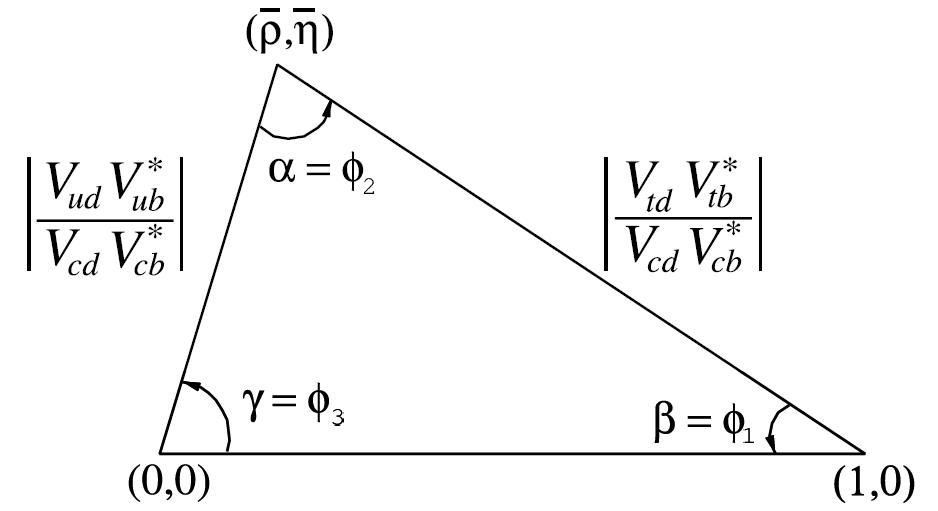
\includegraphics[width=0.49\textwidth]{ckm_triangle}	
	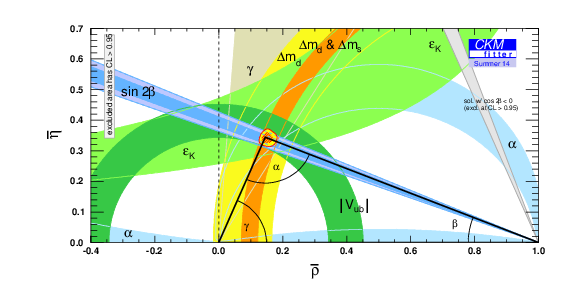
\includegraphics[width=0.49\textwidth]{ckm_fit}	
	\caption{Left: Triangle in the complex $(\bar{\rho}, \bar{\eta})$ plane obtained by the unitarity constraint on the CKM matrix in equation (\ref{eq:triangle}). Right: Current status of the CKM matrix with all measured variables included. Figures taken from \cite{PDG} and \cite{CKM_fitter}
    respectively.}
	\label{fig:CKM_triangle}
\end{figure}

\section{The measurement of \CP violation in mixing with \asld}
The symmetry transformation \CP describes

\section{Methods of parameter estimation}
This section briefly describes two methods to estimate parameters, which are used in this thesis.

\subsection{Maximum-Likelihood method}
A common task in High Energy Physics is to find the best estimate for a set of parameters $\vec{\theta}$ by a measurement of some variables $\vec{x}$.
As an example one wants to measure the mass $m_X$  and the width $\Gamma_X$ of a particle $X$ decaying into two daughter particles $A$ and $B$, i.e. $X \to AB$.
For this purpose one would measure the energies $E$ and momenta of $p$ multiple times.
Thus the set of measured variables would be $\vec{x} = (E_A, \vec{p}_A, E_B, \vec{p}_B)$ and one would try to find the ``best" value for the parameters $\vec{\theta} = (m_X, \Gamma_X)$. 
The most frequently used method for the estimate of $\vec{\theta}$ is the \textsc{Maximum-Likelihood Method}.
Given a theoretical prediction of the measured distribution in form of a probability density function $f(\vec{x}|\vec{\theta})$ one can define the likelihood function
\begin{align}
    \mathcal{L}(\vec{x}|\vec{\theta}) := \prod_{i=1}^{N} f(\vec{x}_i|\vec{\theta}),
\end{align}
where $N$ denotes the number of (independent) measurements.
The maximum of this likelihood function $\mathcal{L}$ with respect to $\vec{\theta}$ is assumed to be the best estimate of $\vec{\theta}$.
Practically one minimises equivalently $-\log(\mathcal{L})$ for computational reasons.

Often, a probability density function $P$ is a linear combination of several components, e.g. a signal and background component $P_\text{sig}$ respectively $P_\text{bkg}$.
Thus the number of events $N$ is a random variable as well.
If $N$ obeys the Poisson distribution the so-called \textsc{Extended Likelihood Function} can be defined as: 
\begin{align}
    &\mathcal{L}_\text{ext}(\vec{x} | \Nsig, \Nbkg, \vec{\theta}) :=  \nonumber \\ 
    &\qquad \frac{(\Nsig+\Nbkg)^N\exp{(\Nsig+\Nbkg)}}{N!} \prod_{i=1}^{N} \left[f_\text{sig}P_\text{bkg}(\vec{x}_i|\vec{\theta}) + f_\text{bkg}P_\text{bkg}(\vec{x}_i|\vec{\theta})\right],
\end{align} 
where $N_j$ denotes the corresponding yield and $f_j:=\frac{N_j}{N}$ the fraction of signal respectively background component.
Thus the maximisation of the extended likelihood function $\mathcal{L}_\text{ext}$ enables to estimate the yields of each component at the same time \cite{Lista_Statistics, PDG}.

\subsection{Beeston-Barlow method}
\label{sec:BeestonBarlow}
When one tries to estimate the composition of a data sample it might happen that there does not exist an analytic form of the distribution.
Thus, one relies on simulations and has to bin the data into $n$ bins.
This gives a set of numbers ${d_i}$ with $i \in [1,n]$, where $d_i$ denotes the number of data events in falling into bin $i$.
Let $j$ denote a source contained in the data, $P_j$ its strength and $a_{ji}$ the number of simulated events from source $j$ in bin $i$, then the predicted number of events in bin $i$ is given by
\begin{align}
    f_i := N_\text{D} \sum_{j=1}^{m} \frac{P_j a_{ji}}{N_j},
\end{align}
where $N_\text{D}$ is the total number of events in the data sample, $N_j$ the number of simulated events for source $j$ and $m$ the number of sources.
Starting from a Poisson distributed probability of observing a particular $d_i$ as
\begin{align}
    \mathrm{e}^{f_i} \frac{f_i^{d_i}}{d_i!}
\end{align}
the logarithmic likelihood to be maximised looks like
\begin{align}
    \log \mathcal{L} = \sum_{i=1}^{n} \left[d_i \log(f_i) - f_i\right] \label{eq:BinnedLL}
\end{align}
after dropping the constant factorials.
This likelihood function is also known as \textsc{Binned Likelihood}.

Nonetheless, the binned likelihood of equation (\ref{eq:BinnedLL}) does not account for finite sizes of the simulation samples.
Due to large computation times simulation samples are often small and there are non-negligible statistical fluctuations in the $a_{ji}$.
Thus the likelihood function has to be modified as follows:
The predicted number of events in a bin is now
\begin{align}
    f_i := N_\text{D} \sum_{j=1}^{m} \frac{P_j A_{ji}}{N_j},
\end{align}
where $A_{ji}$ is the unknown expected number of events for source $j$ in bin $i$.
The ``observed" $a_{ji}$ in the simulation sample is generated from $A_{ji}$ by a Poisson distribution\footnote{Actually, the $a_{ji}$ obey a binomial distribution. However, for $A_{ji} << N_j$ it can be approximated by a Poisson distribution.}.
Thus, the probabilities of observing a set of ${d_i}$ and ${a_ji}$ have to be combined and the likelihood function to be maximised is
\begin{align}
    \log \mathcal{L} = \sum_{i=1}^{n} \left[d_i \log(f_i) - f_i\right] + \sum_{i=1}^{n} \sum_{j=1}^{m} \left[a_{ji} \log(A_{ji}) - A_{ji}\right]. \label{eq:BBLL}
\end{align}
Throughout this analysis, the maximisation of this likelihood function in equation (\ref{eq:BBLL}) is referred to as \textsc{Beeston-Barlow Method} \cite{BeestonBarlow}.
